\chapter{Finite element method}
\label{ch:Finite_element_method}

%El calculo variacional es una disciplina que se encarga de encontrar el minimo de un funcional. En donde un funcional es el mapeo de un espacio vectorial a los reales. Si esta es la ecuacion diferencial
%
%Lu = f
%
%Entonces el residuo es
%
%R(v) = Lv - f
%
%y si se evalua en la solucion u
%
%R(u) = 0
%
%entonces minimizar un residio no tiene gracia, porque se trata de encontrar la solucion exacta a la ecuacion diferencial. Que es lo que no sabemos hacer. Pero entonces podemos proponer minimizar un residuo promediado, p. ej., la norma del error. Entonces definimos un residuo ponderado
%
%Rp(u,v) = int(v*Lu - v*f)
%
%(weigthin se dice ponderar en espanhol). Entonces, uno propone una solucion con una forma conocida: senos y cosenos, polinomios, Gaussianas... Y encuentra la combinacion lineal de esas funciones que minimiza Rp (Y a estamos hablando de metodos aproximados para resolver la ecuacion diferencial).

The Finite Element Method approximates an integral formulation that is --in some sense-- equivalent with a differential equation. This integral (weak) formulation can be obtained from a variational principle, such as the Principle of Virtual Works, or the Integral of Action \cite{Goldstein2001}, but can also be obtained from a more general approach like the Weighted Residuals Method \cite{Zienkiewicz2005, Reddy_functional_analysis}. In the case of electromagnetic waves, we can formulate a variational principle where the functional to be minimized is the energy carried by the electric and magnetic fields defined in \ref{eq:energy_functional}. 

This project uses the Galerkin Finite Element Method to construct an approximate solution of  initial-boundary value and eigenvalue problems involving the wave equation of electromagnetic fields \ref{eq:E-wave-harmonic2}. Galerkin's method is one of these weighted residual methods in which both the weight functions and the bases for approximating the solution are defined as a linear combination of piece wise continuous polynomial functions $h$: $$u = \sum_{i=1}^Nu_ih_i.$$ Where $u_i$ are the unknown expansion coefficients and $h_i$ are the base functions. 

So if we have a general partial differential equation of the form: 
\begin{equation}
\mathcal{L}(u) = f,
\label{eq:general_form_of_DE}
\end{equation}  where $\mathcal{L}$ denotes a differential operator, $u$ denotes the unknown solution to be found and $f$ denotes source function, we can assume an approximation $u'$ of $u$ and build a residual defined as $\mathcal{R} = \mathcal{L}(u')-f$ to be minimized. What we want is to find a function $u'$ that makes $\mathcal{R}$ a minimum in an \emph{average} sense. A way to do this is to construct a functional that is defined as the integral over all space of the residual multiplied by a weighting function $w$, and then set this functional equal to zero 
\begin{equation}
\int w \mathcal{R}(u') = 0.
\end{equation}
Now depending on what bases we use to approximate $u$ and what we choose to do with the weighting functions we will get a different weighted residual method to obtain $u$. 
Galerkin's method works by defining $w$ in the same form of $u$ as shown before.

In the rest of this chapter, we will show how to apply Galerkin's Finite Element formulation to electromagnetism problems, and specifically to the time harmonic wave equation described in \ref{eq:E-wave-harmonic2} without sources. The concepts treated here are the basis of the code that has been implemented in the software platform PeyeQM that will be introduced in the following chapter.

\section{Weak formulation of the problem}

As mentioned before, in a weighted residual formulation weight functions  are used in order to minimize a functional that is stated as the integral of the operator problem over a given  simulation domain such as the one illustrated in figure \ref{fig:domain}. 

\begin{figure}[h]
\centering
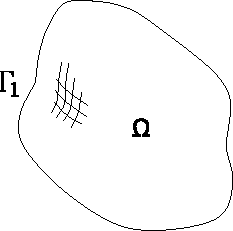
\includegraphics[height=5cm]{./img/dominio.pdf}
\caption{Abstract representation of a simulation domain $\Omega$ and its boundary $\Gamma$}
\label{fig:domain}
\end{figure}

If the field we want to obtain $\mathbf{E}$ is solution to equation \ref{eq:E-wave-harmonic2}, then it must satisfy the variational form that results by multiplying \ref{eq:E-wave-harmonic2} by an arbitrary test function $\mathbf{W}$ and then integrating over $\Omega$ $\int_{\Omega} \mathbf{W} \cdot$(\ref{eq:E-wave-harmonic2}):

\begin{equation}
\int_{\Omega}\mathbf{W}\cdot\left[ \nabla\times\ \left(\mu_r^{-1}\nabla\times \mathbf{E} \right) - k_0^{2}\epsilon_r\cdot \mathbf{E}\right]= 0. \label{eq:E-wave-harmonic3} 
\end{equation}
Note that here the term $\nabla\times\ \left(\mu_r^{-1}\nabla\times \bullet \right) - k_0^{2}\epsilon_r\cdot \bullet$ stands as the operator $\mathcal{L}$ in equation \ref{eq:general_form_of_DE}. and $f=0$. Separating the two terms of this new $\mathcal{L}$ we get:
\begin{equation}
\int_{\Omega}\mathbf{W}\cdot \nabla\times\ \left(\mu_r^{-1}\nabla\times \mathbf{E} \right) -k_0^{2}\int_{\Omega}\mathbf{W}\cdot \epsilon_r\cdot \mathbf{E}= 0. \label{eq:E-wave-harmonic4} 
\end{equation}
Now, lets focus on the first integral on the left hand side of the equation. Here we will invoke the vector identity: $\mathbf{A}\cdot\nabla\times\mathbf{B} = \mathbf{B}\cdot\nabla\times\mathbf{A} - \nabla\cdot(\mathbf{A}\times\mathbf{B}.)$ 
Where $\mathbf{A}=\mathbf{W}$ and $\mathbf{B}=\epsilon_r\nabla\times \mathbf{E}$ To express it as:

\begin{equation}
\int_{\Omega}\mathbf{W}\cdot \nabla\times\ \left(\mu_r^{-1}\nabla\times \mathbf{E} \right) = \int_{\Omega} \mu_r^{-1}\nabla\times \mathbf{E}\cdot \nabla\times\mathbf{W}-\int_{\Omega}\nabla\cdot
\left(\mathbf{W}\times\mu_r^{-1}\nabla\times\mathbf{E}\right). 
\end{equation}

The Divergence Theorem allows us to transform the volume integral on the second term of the right hand side to a closed surface integral:

\begin{equation}
\int_{\Omega}\nabla\cdot
\left(\mathbf{W}\times\mu_r^{-1}\nabla\times\mathbf{E}
\right) = \oint_{\Gamma}\hat{n}\cdot
\left(\mathbf{W}\times\mu_r^{-1}\nabla\times\mathbf{E}
\right).
\end{equation}

And we will have two kinds of boundaries, Dirichlet and Neumann \cite{Garcia2011}, thus $\oint_{\Gamma} = \int_{\Gamma_D}+\int_{\Gamma_N}$. Weight functions have been conveniently chosen to be zero at Dirichlet boundaries so, $\mathbf{W}\mid_{\Gamma_D}=0$. 
One last step is to apply the triple product identity to the argument inside the Neumann integral so that:

$$\hat{n}\cdot
\left(\mathbf{W}\times\mu_r^{-1}
\nabla\times\mathbf{E}\right) =\mathbf{W} \cdot
 \left(\mu_r^{-1}\nabla\times\mathbf{E}\times\hat{n}\right) = -\mathbf{W} \cdot
 \left(\hat{n}\times\mu_r^{-1}
\nabla\times\mathbf{E}\right).$$

Substituting everything we get the form:

\begin{equation}
\int_{\Omega} \mu_r^{-1}\nabla\times \mathbf{E}\cdot \nabla\times\mathbf{W}
-k_0^{2}\mathbf{W}\cdot \epsilon_r\cdot \mathbf{E}
+ \int_{\Gamma_N} \mathbf{W} \cdot
 \left(\hat{n}\times\mu_r^{-1}
\nabla\times\mathbf{E}\right)
= 0. \label{eq:E-wave-weak} 
\end{equation}


\section{Boundary conditions}

For uniqueness of the solution and given that this is a boundary value problem, we must define how is the field or the derivative of the field at boundaries. The two conditions we come upon for defining how the system behaves at boundaries $\Gamma_D$ and $\Gamma_N$ are:
\begin{align}
\hat{n}\times\mathbf{E}&=\mathbf{P} \quad on \ \Gamma_D,\\
\hat{n}\times\left(\bar{\bar{\mu_r}}^{-1}
\nabla\times \mathbf{E}\right) &=\mathbf{K}_N \quad on \ \Gamma_N. \label{eq:BC}
\end{align}
$\mathbf{P}$ is the value for tangential electric field on Dirichlet boundaries $\Gamma_D$,  and $\mathbf{K}_N$ is a function that represents boundary sources or electric field flux on $\Gamma_N$.

Replacing equation \ref{eq:BC} in \ref{eq:E-wave-weak} we get:

\begin{equation}
\begin{array}{rcl}
\int_{\Omega} \mu_r^{-1}\nabla\times \mathbf{E}\cdot \nabla\times\mathbf{W}
-k_0^{2}\mathbf{W}\cdot\epsilon_r\cdot \mathbf{E}
&=& - \int_{\Gamma_N} \mathbf{W} \cdot\mathbf{K}_N,  \label{eq:E-wave-weak_3} 
\end{array}
\end{equation}

by using:
$$-\mathbf{W}\cdot\left(\hat{n}\times \left( \hat{n}\times 
\mathbf{E} \right)\right)  = \left(\hat{n}\times \mathbf{W}\right)\cdot\left( \hat{n}\times 
\mathbf{E} \right). $$


\section{Abstract form of the equation}

Now, in order to reduce verbosity and ease the calculations, we define a set of bi-linear operators\footnote{Which are similar to the definition of inner product made in \ref{eq:inner_prod}} who represent the integrals in \ref{eq:E-wave-weak_3}. These operators are meant to ease mathematical manipulations. Let's do some definitions first:
$\mathbb{V}$ is a vector space of square integrable functions that vanishes at Dirichlet boundaries.

$$ \mathbb{V}=\left\lbrace v\in L^2(a,b):a(v,v)<\infty\wedge v(\Gamma_D)=0\right\rbrace,$$
$$L^2 =\left\lbrace v: \Omega \rightarrow \mathbb{R}\quad such \ that\quad \int_{\Omega}v^2d\Omega =0\right\rbrace.$$ 
Operator $a$, represents the first term of the left hand side in equation \ref{eq:E-wave-weak_3}:
\begin{equation}
\begin{array}{rcl}
      a(\mathbf{W},\mathbf{E})&&:\mathbb{V}\times \mathbb{V}\rightarrow \mathbb{R},\\
      a(\mathbf{W},\mathbf{E})&&= \int\limits_{\Omega}\mu_r^{-1}\nabla\times \mathbf{E}\cdot \nabla\times\mathbf{W} d\Omega,
\label{eq:a_def}
\end{array}
\end{equation}
$b$ is the second term in the left hand side in equation \ref{eq:E-wave-weak_3}:
\begin{equation}
\begin{array}{rcl}
      m(\mathbf{W},\mathbf{E})&:\mathbb{V}\times \mathbb{V}\rightarrow \mathbb{R},\\
      m(\mathbf{W},\mathbf{E})&= \int\limits_{\Omega} k_0^{2}\mathbf{W}\cdot \epsilon_r\cdot \mathbf{E} d\Omega,
\label{eq:m_def}
\end{array}
\end{equation}
$q$ represents boundary sources.
\begin{equation}
\begin{array}{rcl}
      q(\mathbf{W})&:\mathbb{V}\rightarrow \mathbb{R},\\
      q(\mathbf{W})&=\int_{\Gamma_N} \mathbf{W} \cdot\mathbf{K}_N.
\label{eq:m_def}
\end{array}
\end{equation}
%and $f$ body source terms. In the implementation $f=0$.
%\begin{equation}
%\begin{array}{rcl}
%      f(\mathbf{W})&:\mathbb{V}\rightarrow \mathbb{R}\\
%      f(\mathbf{W})&=ik_0Z_0 \int_{\Omega} \mathbf{W}\cdot\mathbf{J}
%\label{eq:m_def}
%\end{array}
%\end{equation}
Where $\mathbf{K}_N$ is a are known boundary condition.
These operators take vectors as inputs and return scalars. Using them one can construct a form of equation \ref{eq:E-wave-weak_3} known as the abstract form:

\begin{equation}
a(\mathbf{W},\mathbf{E}) - m(\mathbf{W},\mathbf{E}) = -f(\mathbf{W})-q(\mathbf{W})
\label{eq:abstract_E_wave}.
\end{equation}

\section{Base functions and discretization}
However right now we don't have a proper Galerkin formulation because $\mathbf{E}$ is still a continuous function of all space, and thus, very hard to solve. Specifically if we are in a 2D domain where:
\[\mathbf{E}=E(x,y)_x\hat{a}_x + E(x,y)_y \hat{a}_y. \]
To have a discrete problem to solve for $\mathbf{E}$, it must be approximated, and this is done by assuming that we can write it as a linear combination of base functions. Obviously,  to have a computable problem we must take only a finite number of those base functions. What we do in FE is using piecewise polynomials as base functions, piecewise polynomials are functions that we define continuous only over disjoint finite regions of space. So a function like $\mathbf{E}$ that is continuous over all space can be split into a number $N$ of functions that each is continuous over a finite region of the domain. 
Being so, the first step is to split the domain into elements like illustrated in figure \ref{fig:disc_domain}. Each base function of the expansion will exist only within its corresponding finite region or element. With that we have
\begin{equation}
\mathbf{E} = \sum_{el=1}^{N_{el}}\mathbf{E}^{el}.
\end{equation}
Where $\mathbf{E}^{el}$ is a linear combination of interpolation functions $h_i$ who are locally continuous inside elements $el$:
\begin{equation}
\mathbf{E}^{el} = \sum_{i =1}^N E_i^{el}h_i^{el},
\end{equation}
and the values $E_i^{el}$ are the expansion coefficients that allow the functions to reach $\mathbf{E}$.
\begin{figure}
\centering
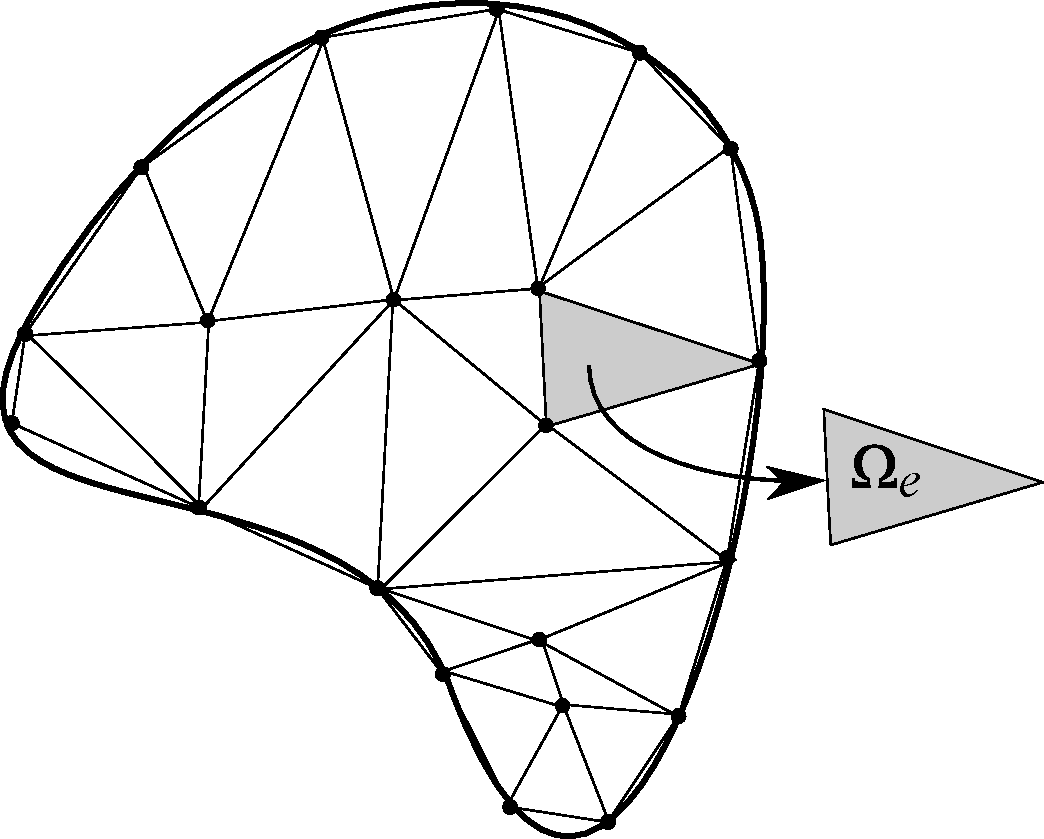
\includegraphics[scale=0.3]{./img/dominio_discreto.pdf}
\caption{Discretized domain defined by a set of elements and their nodes. Taken with permission from \cite{Guarin2012}}
\label{fig:disc_domain}
\end{figure}
Now, these functions $h_i$ can be seen as local interpolation functions of arbitrary order, and the order of the function will be proportional to the number of evaluation points in space needed to define it. The points will herein be called nodes, and they are a discrete representation of the coordinates in the domain. For higher order bases, one needs more evaluation points to define them, and because its easier to solve for lower order polynomials (fewer unknowns) we intentionally limit their order (usually to first or second order). Notice that an exact representation of $\mathbf{E}$ happens when $N\leftarrow\infty$.

\begin{figure}
\centering
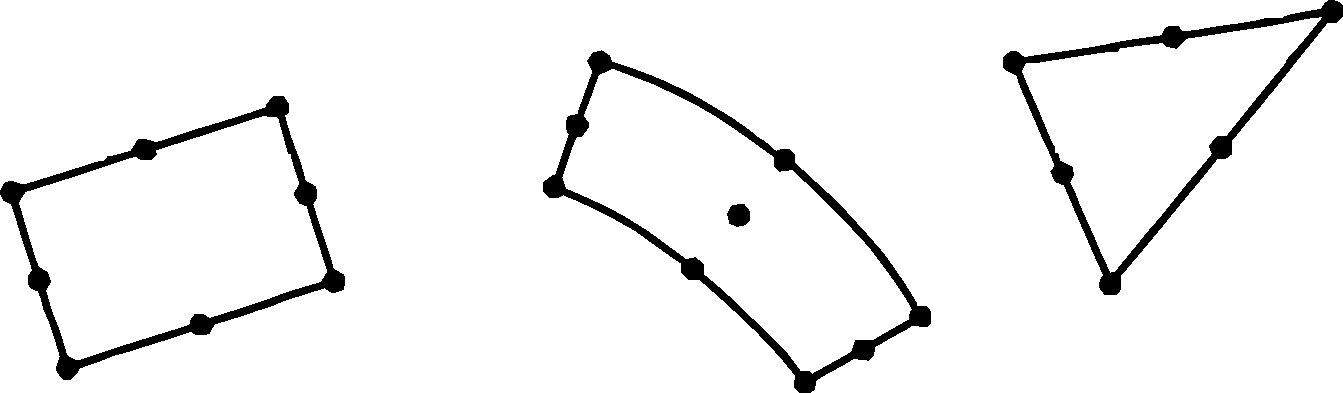
\includegraphics[scale=0.5]{./img/two_dim_elem.pdf}
\caption{Three examples of commonly used two-dimensional elements. The one on the center is a 9 node quadrilateral element with a complete basis. To the left is a serendipity QUAD8 elements with 8 nodes, and to the right a 6 node triangular element.\cite{Bathe1996}}
\label{fig:2d_elem}
\end{figure}

For bi-dimensional elements like those in \ref{fig:2d_elem} one has to define one interpolation function for each node and they must be built so that on each node $i$ the function $h_i$ takes the value of 1 and zero at the rest. This is accomplished for a quadrilateral element of 4 to 9 nodes by using the functions given in table \ref{tab:int_funct}. The elements used in the software for the solution of electromagnetic fields are 8 node quadrilateral elements.
\begin{figure}
\centering
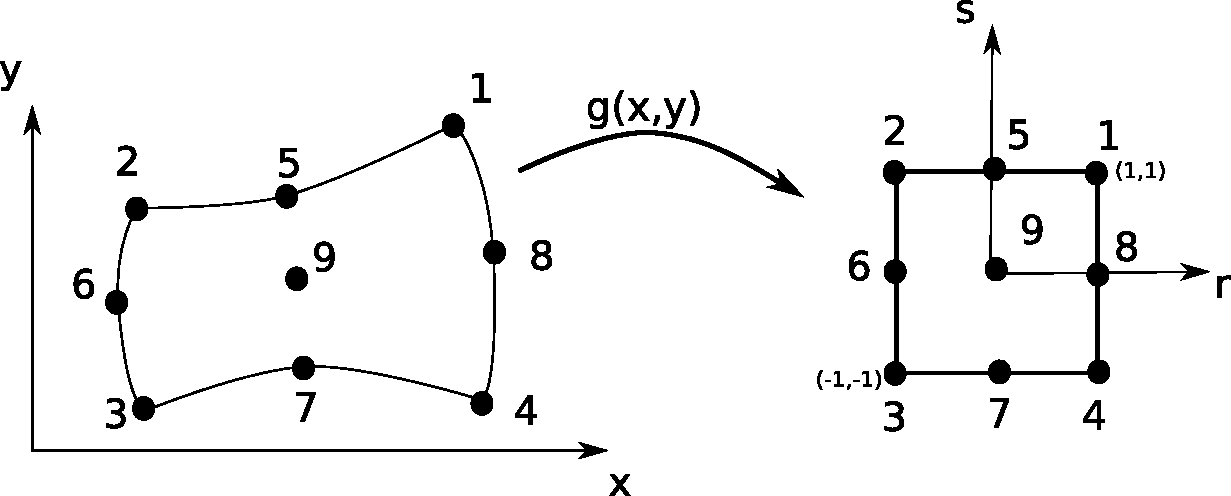
\includegraphics[scale=0.5]{./img/2D_gen_elem.pdf}
\caption{In order to ease the definition of base functions, every element is transformed to a generalized ``isoparametric element'' by means of a function $g(x,y)$ \cite{Bathe1996} so that all elements share the same base. The element on the left has an arbitrary shape and position, and by means of function $g(x,y)$ is mapped to a standard element in a domain in $r$, $s$ that goes from $-1$ to $1$. }
\end{figure}

\begin{center}
\begin{table}
\centering
    \begin{tabular}{r|c|c|c|c|c|c|}
       \multicolumn{2}{c}{~} & \multicolumn{5}{c}{Include if the node is present.}\\
       \multicolumn{1}{c}{~} & \multicolumn{1}{c|}{~} & $i=5$ & $i=6$ & $i=7$ & $i=8$ & $i=9$ \\      
    $h_1$ & $\frac{1}{4}\left(1+r\right)\left(1+s\right)$    & $-\frac{1}{2}h_5$ & ~     & ~ & $-\frac{1}{2}h_8$ & $-\frac{1}{2}h_9$ \\
    $h_2$ & $\frac{1}{4}\left(1-r\right)\left(1+s\right)$    & $-\frac{1}{2}h_5$ & $-\frac{1}{2}h_6$     &  &  & $-\frac{1}{2}h_9$ \\
    $h_3$ & $\frac{1}{4}\left(1-r\right)\left(1-s\right)$    &     & $-\frac{1}{2}h_6$ & $-\frac{1}{2}h_7$ &  & $-\frac{1}{2}h_9$ \\
    $h_4$ & $\frac{1}{4}\left(1+r\right)\left(1-s\right)$    &      &      & $-\frac{1}{2}h_7$ & $-\frac{1}{2}h_8$ & $-\frac{1}{2}h_9$ \\
    $h_5$ & $\frac{1}{2}\left(1-r^2\right)\left(1+s\right)$  &  & & &  & $-\frac{1}{2}h_9$ \\
    $h_6$ & $\frac{1}{2}\left(1-s^2\right)\left(1-r\right)$  & & &  &  & $-\frac{1}{2}h_9$ \\
    $h_7$ & $\frac{1}{2}\left(1-r^2\right)\left(1-s\right)$  & & & & &$-\frac{1}{2}h_9$ \\
    $h_8$ & $\frac{1}{2}\left(1-s^2\right)\left(1+r\right)$  & & & & & $-\frac{1}{2}h_9$ \\
    $h_9$ & $\frac{1}{2}\left(1-r^2\right)\left(1-r^2\right)$& & & & & $-\frac{1}{2}h_9$\\
    \end{tabular}
\caption{Interpolation functions of four to nine variable-number-nodes two-dimensional isoparemtric elements.}
\label{tab:int_funct}
\end{table}
\end{center}
We will proceed by presenting some notation definitions for the future development:
Lets say that the set of nodes that represent values of the field in the domain is called $\eta$. On nodes belonging to Dirichlet boundaries we will know the value of the field ($\mathbf{P}$) and it is convenient to split the set of nodes into its known and unknown elements $\eta_D\cup\eta\setminus\eta_D=\eta$.  Each physical node will contain two components of the field\footnote{In a vectorial element formulation like the one used for EM fields in our program.}, one for $x$ and the other for $y$. So the number of evaluation nodes gets doubled.

If $N$ is the total number of values:

\[N = n_x + n_y,\]

where $n_x$ and $n_y$ are the number of evaluation nodes associated to fields in $x$ and  $y$	. When programming it is convenient to distinguish where does a node belongs, so we will treat $n_x$ and $n_y$ as sets as well in order to build a notation for the sums based on  how an iterator surfs a set.


\begin{align*}
n_x &= n_x \in \eta_D + n_x \in \eta\setminus\eta_D,\\
n_y &= n_y \in \eta_D + n_y \in \eta\setminus\eta_D.
\end{align*}
If we say: $$i: n_x\in \eta_D,$$  that will mean that the iteration will occur on the indexes that belong to the set of nodes in the Dirichlet region associated to $x$ component of the field. The field for each node, for each region and and for each component can then be approximated by:

\begin{align*}
E(x,y)_x\approx \sum_{i:\ n_x \in \eta_D} h_i E_i^x+\sum_{i:\ n_x \in \eta\setminus\eta_D} h_i E_i^x,\\
E(x,y)_y\approx \sum_{i:\ n_y \in \eta_D}h_iE_i^y+
\sum_{i:\ n_x \in \eta\setminus\eta_D}h_iE_i^y.
\end{align*}
 
Left side are known values and right side unknowns.
In the same way for test functions $W$ on the boundary we have: 
\[\mathbf{W}=W(x,y)_x\hat{a}_x + W(x,y)_y \hat{a}_y, \]
\begin{align*}
W(x,y)_x\approx \sum_{i:\ n_x \in \eta_D} h_i W_i^x+\sum_{i:\ n_x \in \eta\setminus\eta_D} h_i W_i^x, \\
W(x,y)_y\approx \sum_{i:\ n_y \in \eta_D}h_iW_i^y+
\sum_{i:\ n_x \in \eta\setminus\eta_D}h_iW_i^y.
\end{align*}
Moreover $\mathbf{K}_N$ can also be interpolated if there are Neumann boundary conditions: 
%\[\mathbf{J}=J(x,y)_x\hat{a}_x + J(x,y)_y \hat{a}_y \]
%
%\begin{align*}
%J(x,y)_x\approx \sum_{i:\ n_x \in \eta_D}h_i J_i^x+\sum_{i:\ n_x \in \eta\setminus\eta_D}h_i J_i^x \\
%J(x,y)_y\approx \sum_{i:\ n_y \in \eta_D}J_i^y+
%\sum_{i:\ n_x \in \eta\setminus\eta_D}J_i^y
%\end{align*}
$$\mathbf{K}_N=K(x,y)_x\hat{a}_x + K(x,y)_y \hat{a}_y,$$
\begin{align*}
K(x,y)_x\approx \sum_{i:\ n_x \in \eta_D}h_i K_i^x+\sum_{i:\ n_x \in \eta\setminus\eta_D} 0, \\
K(x,y)_y\approx \sum_{i:\ n_y \in \eta_D}h_i K_i^y+
\sum_{i:\ n_x \in \eta\setminus\eta_D} 0.
\end{align*}

Substitution of $\mathbf{E}$ and $\mathbf{W}$, into \ref{eq:E-wave-weak_3} is a mess. To make it easier lets use the operators and their properties. To be bi linear is to be linear in both arguments, to be linear means to satisfy \href{http://en.wikipedia.org/wiki/Additive_function}{additivity} and \href{http://en.wikipedia.org/wiki/Homogeneous_function}{homogeneity}. An illustration of this:

\begin{align*}
\alpha (u+\beta v, w)&=\alpha a(u,w)+\beta a(v,w),\\
a(u,\alpha v+\beta w)&=\alpha a(u,v)+\beta a(u,w).
\end{align*}

The rotational and dot product inside the integrals defined in the abstract forms are linear. A proof for that is out of the reach of this document. 
The proof of
\[a(u,v) = a(v,u),\]
was made in equation \ref{eq:hermiticity_proof}, and a proof of
\[m(u,v) = m(v,u),\]
is obtained by assuming that $v$ and $u$ have the same base, which we did by using the Galerkin weighting.

So the following can happen:

\begin{align}
a\left(W_x,E_x\right)&=& a\left( \sum_{i:\ n_x \in \eta_D} h_i W_i^x, \sum_{j:\ n_x \in \eta_D} h_j E_j^x\right)+a\left(\sum_{i:\ n_x \in \eta\setminus\eta_D} h_i W_i^x,\sum_{j:\ n_x \in \eta\setminus\eta_D} h_j E_j^x\right)\nonumber, \\
&=&  \sum_{i:\ n_x \in \eta_D}W_i^x a\left(  h_i , \sum_{j:\ n_x \in \eta_D} h_j E_j^x\right)+\sum_{i:\ n_x \in \eta\setminus\eta_D} W_i^x a\left( h_i,\sum_{j:\ n_x \in \eta\setminus\eta_D} h_j E_j^x\right)\nonumber,\\
&=&\sum_{i:\ n_x \in \eta_D}W_i^x \sum_{j:\ n_x \in \eta_D}E_j^x a\left(  h_i ,  h_j \right)+\sum_{i:\ n_x \in \eta\setminus\eta_D} W_i^x \sum_{j:\ n_x \in \eta\setminus\eta_D}  E_j^x a\left( h_i, h_j \right)\nonumber,\\
&=& \sum_{j:\ n_x \in \eta_D} a\left(  h_i ,  h_j \right)E_j^x \sum_{i:\ n_x \in \eta_D}W_i^x+\sum_{j:\ n_x \in \eta\setminus\eta_D}   a\left( h_i, h_j \right)E_j^x\sum_{i:\ n_x \in \eta\setminus\eta_D} W_i^x \label{eq:substitution_of_app_fields_in_a}.
\end{align}

\[\sum_{j:\ n_x \in \eta_D}E_j^x = \vec{g}_j^x, \]
\[\sum_{i:\ n_x \in \eta\setminus\eta_D}W_i^x = \vec{W}^x,\]
\[\sum_{j:\ n_x \in \eta\setminus\eta_D}E_j^x = \vec{E}^x, \]
\[\vec{g}_i = \vec{g}_j^x+\vec{g}_j^y \qquad j = 1.. N, \]
$\vec{g}_j$ is a vector of size $N$ that holds values of $E$ on each Dirichlet boundary node for both $x$, and $y$ components. Vector $\hat{g}_i^y$ follows from a similar procedure on $E_y$. It is of importance to say that even though the sets defined under the summation are subsets of the set of all nodes, when programming, their associate vectors will span the whole domain. In other words this notation stands for entries to indexes to vectors that may be defined full of zeroes. Or in a different approach: $j$ in $j:\ n_x \in \eta_D$ can be indexes 1 and $N$ meaning that the first and last nodes belong to Dirichlet boundary points on $x$. All other elements of the vector are undefined and hold their initiation value zero.


Changing the indexes $i$, $j$ and using the definition of \href{http://en.wikipedia.org/wiki/Dot_product}{dot product} in a matrix notation we can translate the abstract form as:

\begin{align*}
a\left(W_x,E_x\right)=&\langle \mathbb{A}\vec{g}^x,\vec{W}^x\rangle
+\langle\mathbb{A}\vec{E}^x,\vec{W}^x\rangle . 
\end{align*}

Where $\mathbb{A}$ is a matrix whose elements contain the indexed integration over the basis functions $h_i$, and $h_j$, these are known values because we know the form of the functions and can calculate the integrals by numerical or analytic means. For the solution in the software routines we implemented numerical integration based on Gauss-Legendre quadrature as defined in \cite{Bathe1996}. 

Matrix $\mathbb{A}$ is known as the stiffness matrix in Mechanics, and here it relates to energy stored in form of electric field. Matrix $\mathbb{A}$ is built as a combination of matrices $\mathbb{A}^x$ and $\mathbb{A}^y$:
\[\mathbb{A} = \mathbb{A}^x+\mathbb{A}^y,\]
where
\[\mathbb{A}^x = \sum_{i,j}^{n_x \in \eta\setminus\eta_D} a(h_i,h_j)+\sum_{i,j}^{n_y \in \eta\setminus\eta_D} a(h_i,h_j).\]

The product $\mathbb{A}^x\vec{g}^x = \vec{d}^x$ will be called the Dirichlet vector.
\begin{align}
a\left(W_x,E_x\right)=&\langle \vec{d}^x,\vec{W}^x\rangle
+\langle\mathbb{A}^x\vec{E}^x,\vec{W}^x\rangle. \label{eq:potential_discrete} 
\end{align}

In a very similar way but now substituting the approximate functions into the kinetic operator $m(\mathbf{W},\mathbf{E})$ we get:

\begin{align}
m\left(W_x,E_x\right)=&\langle \mathbb{M}^x\vec{g}^x,\vec{W}^x\rangle
+\langle\mathbb{M}^x\vec{E}^x,\vec{W}^x\rangle\nonumber, \\
m\left(W_x,E_x\right)=&\langle \vec{b}^x,\vec{W}^x\rangle
+\langle\mathbb{M}^x\vec{E}^x,\vec{W}^x\rangle. \label{eq:kinetic_discrete}
\end{align}

With $\mathbb{M}$ as the mass matrix or inductance matrix. Being related to the time derivative of the electric field, we can associate this to energy stored in the form of magnetic fields like a sort of inductance matrix. The global mass matrix is also a combination of terms related to the degree of freedom $x$ and $y$:
\begin{align*}
\mathbb{M} &= \mathbb{M}^x+\mathbb{M}^y,\\
\mathbb{M} &= \sum_{i,j}^{n_x \in \eta\setminus\eta_D} m(h_i,h_j)+\sum_{i,j}^{n_y \in \eta\setminus\eta_D} m(h_i,h_j).
\end{align*}

And the same follows with operator $q$:

\begin{align}
q(W_x) &= \langle \vec{q}^x, \vec{W^x}\rangle \label{eq:newman},\\
\vec{q}_i^x&= \sum_{i:\ n_x \in \eta_N}\int_{\Gamma_N} h_iK_i^x \nonumber.
\end{align}

Where we introduced a subset of the set $\eta  \setminus \eta_D$ called $\eta_N$ which represents nodes on Neumann boundaries.

Substituting definitions: \ref{eq:potential_discrete}, \ref{eq:kinetic_discrete}, \ref{eq:newman}, and \ref{eq:body_source} in equation \ref{eq:abstract_E_wave}, we get:

\begin{align}
\langle\vec{d}^x,\vec{W}^x\rangle
+\langle\mathbb{A}^x\vec{E}^x,\vec{W}^x\rangle-\langle \vec{b}^x,\vec{W}^x\rangle
-\langle\mathbb{M}^x\vec{E}^x,\vec{W}^x\rangle &= -\langle \vec{q}^x, \vec{W^x}\rangle \nonumber,\\
\langle\mathbb{A}^x\vec{E}^x- \mathbb{M}^x\vec{E}^x,\vec{W}^x \rangle &=\langle \vec{b}^x-\vec{d}^x-\vec{q}^x, \vec{W}^x \rangle.
\end{align}

Being $\vec{W}^x$ an arbitrary function, the following linear system of equations appear:
\begin{equation}
\left(\mathbb{A}^x-\mathbb{M}^x\right)\vec{E}^x = \vec{b}^x-\vec{d}^x-\vec{q}^x. \label{eq:harmonic_eq_sys_x}
\end{equation}
Similarly, and following exactly the same procedure:

\begin{equation}
\left(\mathbb{A}^y-\mathbb{M}^y\right)\vec{E}^y = \vec{b}^y-\vec{d}^y-\vec{q}^y. \label{eq:harmonic_eq_sys_y}
\end{equation}


These two systems can be solved simultaneously by intercalating rows and columns of $\mathbb{A}^x$ with $\mathbb{A}^y$, and keeping the formulation as one global matrix multiplying a vector that contains values of the field in both components


\begin{equation*}
\left(\mathbb{A}-\mathbb{M}\right)\vec{E} = \vec{b}-\vec{d}-\vec{q}.
\end{equation*}

Something that is used in many references is to remove rows and columns associated to Dirichlet positions of $E$ in the matrices and vectors of the equation. This is done because we already know the values of $E$ for those points and their information is already saved in vector $\vec{d}$. We will add the symbol $\setminus D$ before the symbols to note that Dirichlet rows and columns should be deleted.

\begin{equation*}
^{\setminus D}\left[\left(\mathbb{A}-\mathbb{M}\right)\vec{E}= \vec{b}-\vec{d}-\vec{q}\right].
\label{eq:harmonic_eq_dirichlet}
\end{equation*}

The solution of this linear system of equations is achieved by means of robust computational routines such as \href{http://www.netlib.org/lapack/}{LAPACK}. And they are finally put together with the known values in order to get a full representation of the field inside the domain.

\section{Edge elements vs Node Elements}
There is another way to represent vector fields in Finite Elements, and it is by using Edge Elements \cite{Jin2010}. Up until now we defined the problem as a simultaneous solution of two scalar fields, one associated to the $x$ coordinate and another to $y$. The advantage of doing that over solving for only one scalar field is that we have much more flexibility in the kinds of boundary conditions that can be formulated. We also achieve higher accuracy and can know more about the problem.

There is  however another form to postulate vector fields, and that is by defining tangential values of the field on each edge and interpolating $\mathbf{E}$ inside the element by using vectorial basis functions, these functions are then not related to each node, but to each line at the element.  In the jargon of Finite Element these are termed Nedelec elements \cite{nedelec1980, kikuchi2001}, some preferences on these elements over the nodal elements resides on the fact that the electric and magnetic fields are 1-manifolds. For example, the field inside  a three node element ($el$) with nodes $1,2,3$ is then the combination of the vector shape functions $\mathbf{N}_{ij}$:
\begin{equation}
\mathbf{E}^{el}(x,y) =\mathbf{N}_{12}^{el}E_{12}^{el} + \mathbf{N}_{13}^{el}E_{13}^{el}+ \mathbf{N}_{23}^{el}E_{23}^{el}.
\end{equation}
And from this point the formulation continues almost identically to what we did before.

There is however an ongoing discussion \cite{Mur1994, Webb1993, Gerr1998} over the advantages and disadvantages of using edge elements instead of nodal elements, and at the moment of implementation edge elements seemed more troublesome to implement than node elements. The formulation of a vector field solver using edge elements is pending as one possible alternative to our current implementation.

\section{Time domain formulation}
For analysis of wave propagation in finite lattices with defects we must be able to simulate the evolution of the fields along time and a stationary harmonic model is no longer suitable. For this, we have to define construct a numerical solution that combines the finite element method and finite differences, the former for the solution of spatial derivatives and the later for time derivatives.
The following procedures are summarized and have less comments because they are made in a very similar way than the process in the previous section.

\subsection{Weak formulation in time dependent problem}
Proceeding in the same way as in the time harmonic case we take equation
\ref{eq:E-wave-loads}, and rewrite it as:
\begin{align}
\nabla\times\left[\mu^-1\cdot\nabla \times\mathcal{E}(t)\right] + \epsilon\cdot\frac{\partial^2 \mathcal{E}(t)}{\partial t^2}=0.
\end{align}

Multiplying by the test function $\mathbf{W}$ and integrating over the entire domain will give us a functional equivalent to \ref{eq:E-wave-weak} to be minimized: 
\begin{align}
\int\limits_{\Omega}\mathbf{W}\cdot\nabla\times\left[\mu^-1\cdot\nabla \times\mathcal{E}(t)\right] + \mathbf{W}\cdot\epsilon\cdot\frac{\partial ^2\mathcal{E}(t)}{\partial t^2}=0,\nonumber\\
\int\limits_{\Omega}\mathbf{W}\cdot\nabla\times\left[\mu^-1\cdot\nabla \times\mathcal{E}(t)\right] +\int\limits_{\Omega} \mathbf{W}\cdot\epsilon\cdot\frac{\partial ^2\mathcal{E}(t)}{\partial t^2}=0 \nonumber,\\
\int\limits_{\Omega} \mu_r^{-1}\nabla\times \mathcal{E}(t)\cdot \nabla\times\mathbf{W}-\int\limits_{\Omega}\nabla\cdot
\left(\mathbf{W}\times\mu_r^{-1}\nabla\times \mathcal{E}(t)
\right) +\int\limits_{\Omega} \mathbf{W}\cdot\epsilon\cdot\frac{\partial ^2\mathcal{E}(t)}{\partial t^2}=0 \nonumber,\\
\int\limits_{\Omega} \mu_r^{-1}\nabla\times \mathcal{E}(t)\cdot \nabla\times\mathbf{W}-\oint_{\Gamma}\hat{n}\cdot
\left(\mathbf{W}\times\mu_r^{-1}\nabla \times\mathcal{E}(t)\right)  +\int\limits_{\Omega} \mathbf{W}\cdot\epsilon\cdot\frac{\partial ^2\mathcal{E}(t)}{\partial t^2}=0 \nonumber,\\
\int\limits_{\Omega} \mu_r^{-1}\nabla\times \mathcal{E}(t)\cdot \nabla\times\mathbf{W}
+\int_{\Gamma_N}\mathbf{W}\cdot
\left(\hat{n}\times\mu_r^{-1}\nabla \times\mathcal{E}(t)\right)
+\int\limits_{\Omega} \mathbf{W}\cdot\epsilon\cdot\frac{\partial ^2\mathcal{E}(t)}{\partial t^2}=0. \label{eq:time_dependent_Electric}
\end{align}

This is achieved remembering that $\hat{n}\cdot\mathbf{W} =0$ on $\Gamma_D$, and using all the vector identities invoked in the previous section.

\subsection{Boundary conditions in time dependent problem}
Boundaries are defined in the same way, but now they are time dependent:
\begin{align}
\hat{n}\times\mathcal{E}(t)=&\mathcal{P}(t)\quad on \quad \Gamma_D,\\
\hat{n}\times\left(\bar{\bar{\mu}}^{-1}\nabla\times\mathcal{E}(t)
\right)+Y\hat{n}\times\left(\hat{n}\times\frac{\partial\mathcal{E} (t)}{\partial t}\right)=& \mathcal{K}_N(t).
\end{align}

Using Neumann boundary conditions applied to \ref{eq:time_dependent_Electric} we get:
\begin{equation}
\int\limits_{\Omega} \bar{\bar{\mu_r}}^{-1}\nabla\times \mathcal{E}(t)\cdot \nabla\times\mathbf{W}
+ \mathbf{W}\cdot\bar{\bar{\epsilon}}\cdot\frac{\partial ^2\mathcal{E}(t)}{\partial t^2}=-\int_{\Gamma_N}\mathbf{W}\cdot\mathcal{K}_N(t). \label{eq:td_weak_form_E_equation}
\end{equation}

\subsection{Base functions and abstract form}
To obtain a finite element solution the spatial domain has to be discretized in the same way as we did when obtaining the frequency domain solution. For this, we use compact support basis functions that in combination with nodal values will give a representation of the global field as the combination of spatial  subdivisions called elements.
In this case is better to invoke the definitions for the approximated functions first-hand:
\begin{align*}
\mathcal{E}(t)=\mathcal{E}(x,y,t)_x\hat{a}_x + \mathcal{E}(x,y,t)_y \hat{a}_y,\\
\mathcal{E}(x,y,t)_x\approx \sum_{i:\ n_x \in \eta_D} h_i \mathcal{E}_i^x(t)+\sum_{i:\ n_x \in \eta\setminus\eta_D} h_i \mathcal{E}_i^x(t),\\
\mathcal{E}(x,y,t)_y\approx \sum_{i:\ n_y \in \eta_D}h_i\mathcal{E}_i^y(t)+
\sum_{i:\ n_x \in \eta\setminus\eta_D}h_i\mathcal{E}_i^y(t).
\end{align*}
Noting that when time derivatives are applied over the field, these will act only on the nodal values $\mathcal{E}_i^x(t)$ so that for example:
\[\frac{\partial \mathcal{E}(x,y,t)_x}{\partial t}\approx \sum_{i:\ n_x \in \eta_D} h_i \frac{\partial \mathcal{E}_i^x(t)}{\partial t}+\sum_{i:\ n_x \in \eta\setminus\eta_D} h_i \frac{\partial\mathcal{E}_i^x(t)}{\partial t}.\]
$\mathbf{W}$ keeps being the same as defined in the previous section.\[\mathcal{J}=\mathbf{J},\]
\[\mathcal{K}_N=\mathbf{K}_N.\]

Operators are almost the same as before. The main difference being that free space related material constants $k_0$ and $Z_0$ haven't been extracted from material matrices $\mu$ and $\epsilon$.

\begin{equation}
\begin{array}{rcl}
      a(\mathbf{W},\mathbf{E})&&:\mathbb{V}\times \mathbb{V}\rightarrow \mathbb{R},\\
      a(\mathbf{W},\mathbf{E})&&= \int\limits_{\Omega}  \bar{\bar{\mu}}^{-1}\nabla\times \mathbf{E}\cdot \nabla\times\mathbf{W} d\Omega,
\label{eq:a_td_def}
\end{array}
\end{equation}
\begin{equation}
\begin{array}{rcl}
      m(\mathbf{W},\mathbf{E})&:\mathbb{V}\times \mathbb{V}\rightarrow \mathbb{R},\\
      m(\mathbf{W},\mathbf{E})&= \int\limits_{\Omega} \mathbf{W}\cdot \bar{\bar{\epsilon}}\cdot \mathbf{E} d\Omega,
\label{eq:m_td_def}
\end{array}
\end{equation}

\begin{equation}
\begin{array}{rcl}
      q(\mathbf{W})&:\mathbb{V}\rightarrow \mathbb{R},\\
      q(\mathbf{W})&=\int_{\Gamma_N} \mathbf{W} \cdot\mathcal{K}_N.
\label{eq:m_td_def}
\end{array}
\end{equation}
%
%\begin{equation}
%\begin{array}{rcl}
%      f(\mathbf{W})&:\mathbb{V}\rightarrow \mathbb{R}\\
%      f(\mathbf{W})&= \int_{\Omega} \mathbf{W}\cdot\frac{\partial\mathcal{J}}{\partial t}
%\label{eq:m_td_def}
%\end{array}
%\end{equation}
Note that all these are operators that act on spatial coordinates and as such are independent of time derivatives. The abstract form for wave propagation in time domain formulation is then:

\begin{equation}
a\left(\mathbf{W},\mathcal{E}\right)+m\left(\mathbf{W},\frac{\partial^2 \mathcal{E}}{\partial t^2}\right)
=-q\left(\mathbf{W}\right).
\end{equation}

If a process of substitution like that shown in equation \ref{eq:substitution_of_app_fields_in_a} is performed for each of these operators, one gets a system of equations equivalent to the one in equation \ref{eq:harmonic_eq_dirichlet}

$$\sum_{j:\ n_x \in \eta_D}\mathcal{E}_j^x = \left\lbrace g^x \right\rbrace, $$
$$ \mathbb{A}^x\left\lbrace g^x \right\rbrace=\left\lbrace d^x \right\rbrace,$$ 
$$\mathbb{M}^x\left\lbrace g^x \right\rbrace=\left\lbrace b^x \right\rbrace,$$
$$\sum_{i:\ n_x \in \eta\setminus\eta_D}W_i^x = \vec{W}^x, $$
$$\sum_{j:\ n_x \in\eta\setminus\eta_D}\mathcal{E}_j^x = \left\lbrace \mathcal{E}^x\right\rbrace, $$
$$\sum_{j:\ n_x \in\eta\setminus\eta_D}\frac{\partial^2 \mathcal{E}_j^x}{\partial t^2} = \frac{\partial^2\left\lbrace \mathcal{E}^x\right\rbrace}{\partial t^2}, $$
%$$ \sum_{i:\ n_x \in \eta}\int_{\Omega} h_i\frac{\partial\mathcal{J}_i^x}{\partial t} = \left\lbrace f^x \right\rbrace, $$
$$\sum_{i:\ n_x \in \eta_N}\int_{\Gamma_N} h_i\mathcal{K}_i^x = \left\lbrace q^x   \right\rbrace,$$

\begin{align}
\langle\left\lbrace d^x \right\rbrace,\vec{W}^x\rangle
+\langle\mathbb{A}^x\left\lbrace\mathcal{E}^x \right\rbrace,\vec{W}^x\rangle&-\langle \left\lbrace b^x \right\rbrace,\vec{W}^x\rangle
-\langle\mathbb{M}^x \frac{\partial^2\left\lbrace\mathcal{E}^x \right\rbrace}{\partial t^2},\vec{W}^x\rangle = -\langle \left\lbrace q^x\right\rbrace, \vec{W^x}\rangle \nonumber,\\
\langle\mathbb{A}^x\left\lbrace \mathcal{E}^x \right\rbrace- \mathbb{M}^x\frac{\partial^2\left\lbrace\mathcal{E}^x \right\rbrace}{\partial t^2},\vec{W}^x \rangle &=\langle \left\lbrace b^x \right\rbrace-\left\lbrace d^x \right\rbrace-\left\lbrace q^x   \right\rbrace.
\end{align}

\begin{equation}
\mathbb{A}\left\lbrace \mathcal{E} \right\rbrace- \mathbb{M}\frac{\partial^2\left\lbrace\mathcal{E} \right\rbrace}{\partial t^2} = \left\lbrace b \right\rbrace-\left\lbrace d \right\rbrace-\left\lbrace q   \right\rbrace-\left\lbrace f\right\rbrace
\label{eq:time_domain_linear_matrix_form}
\end{equation}

In the simulations that were performed as part of the project we did not consider any sources or Neumann boundaries, so $\left\lbrace q=0\right\rbrace$ and $\left\lbrace f\right\rbrace$. The details about the finite difference formulation used to discretize the time derivative are explained in the section (\ref{sec:explicit_formulation}) where the explicit solution of \ref{eq:time_domain_linear_matrix_form} is explored .


\section{Mass matrices}
\label{sec:explicit_formulation}
In numerical methods, and more specifically in Finite elements, mass matrices are a discrete representation of a continuous distribution of something, that multiplies the second time derivative of the solution function.

Mass matrices are cataloged as consistent or diagonal. Consistent mass matrices use the same shape functions as the ones used to generate the element stiffness matrix. All reference to mass matrices mentioned before, were consistent \cite{RobertD.Cook1989}. 
The other way to formulate mass matrices is the lumped mass matrix. Which is made by avoiding the interpolation and simply placing particle masses $m_i$ at nodes $i$ of an element such that $\sum m_i$ is the total element mass. 

The great advantage of lumped mass matrices is that they are diagonal and the solution of the system of equations can be performed in a explicit manner convenient for big computational domains.
However, precision is lost by not stating mass as functions to be interpolated. 

To form a lumped mass matrix one can use the HRZ Lumping scheme 
which consist on the following algorithm \cite{RobertD.Cook1989}:

\begin{enumerate}
\item Compute the diagonal coefficients of the consistent mass matrix.
\item Compute the mass for each element $m$.
\item Compute the trace of the matrix $s$.
\item scale all the diagonal coefficients by multiplying them by the ratio $\frac{m}{s}$.
\end{enumerate}
Lumped mass matrices are used in the implementation of an explicit formulation of Finite Elements in Time Domain FETD where equation \ref{eq:H-wave-homo} is solved instead of \ref{eq:E-wave-harmonic3}. The next section expands on the topic of explicit formulation.

\section{Explicit formulation}

The central-difference method is used to approximate the second order derivative of $\mathbf{E}$ in \ref{eq:time_domain_linear_matrix_form} by expanding $\mathbf{E}_{n+1}$ and $\mathbf{E}_{n-1}$  in taylor series about \add[SEC]{a given discrete} time $n \vartriangle t$:

\begin{equation}
\mathbf{E}_{n+1} = \mathbf{E}_n + \delta t \dot{\mathbf{E}}_n +\frac{\delta t^2}{2} \ddot{\mathbf{E}}_n +\frac{\delta t^3}{6} \dddot{\mathbf{E}}_n+ O(\delta t^4),
\label{eq:2d_taylor_exp1}
\end{equation}
\begin{equation}
\mathbf{E}_{n-1} = \mathbf{E}_n - \delta t \dot{\mathbf{E}}_n +\frac{\delta t^2}{2} \ddot{\mathbf{E}}_n-\frac{\delta t^3}{6} \dddot{\mathbf{E}}_n+ O(\delta t^4).
\label{eq:2d_taylor_exp2}
\end{equation}

Restricting to fourth-order accuracy ($O(\delta t^4)$) and  adding \ref{eq:2d_taylor_exp1} to \ref{eq:2d_taylor_exp2} one can easily solve for $\mathbf{E}_{n+1}$:
\begin{equation}
\ddot{\mathbf{E}}_n = \frac{1}{\delta t^2}\left(\mathbf{E}_{n+1}-2 \mathbf{E}_{n} + \mathbf{E}_{n-1}\right),
\label{eq:central-difference}
\end{equation}
subscript $n$ denotes time $n\delta t$ with $\delta t$ being the selected timestep.

Replacing into our general formulation one gets (fix details):

\begin{equation}
\frac{1}{\delta t^2} \mathbb{M} \mathbf{E}_{n+1} = - \mathbb{A}\mathbf{E}_n + \frac{1}{\delta t^2}\mathbb{M}\left[2
\mathbf{E}_{n}-\mathbf{E}_{n-1}
\right]. 	 
\label{eq:implicit_time_domain}
\end{equation}

The equation \ref{eq:implicit_time_domain} can be solved by an implicit solver that takes matrices and solves in one pass the system of equations for one time $n$ as we do with \ref{eq:harmonic_eq_dirichlet}. This however is not very practical for interesting problems with complex domains when running under workstations that have low memory such as my laptop. For the solution of \ref{eq:implicit_time_domain} is best to solve for each node at a time and this is done by using lumped matrices instead of consistent ones. Having a diagonal mass matrix $\mathbb{M}$ decouples the nodal values in time and makes it possible to solve for $\mathbf{E}_{n+1}$ without solving simultaneous systems of equations. The details of how the algorithm computes the solution of \ref{eq:implicit_time_domain} explicitly are treated in the documentation of the software online.
